\documentclass[../report.tex]{subfiles}
\begin{document}

\chapter{Network architecture: YOLO v3}\label{c:yolo-v3}

\section{YOLO Overview}\label{s:what-is-yolo}
YOLO is a Convolutional Neural Network (CNN) for performing object detection in real-time.\\
CNNs are classifier-based systems that can process input images as structured arrays of data and identify patterns between them.\\
To date, there are two main types of object detection algorithms in the field of deep learning: 
\begin{itemize}
	\item \textbf{Classification-based algorithms} (aka \textit{Two Stage Detectors}): firstly, they select a group of \textit{Region of Interest} (ROI) in the images where the chances that an object is present are high; secondly, they apply Convolutional Neural Networks (CNN) techniques to these selected regions to detect the presence of an object.
	\begin{itemize}
		\item a problem associated with these types of algorithms is that they need to execute a detector in each ROI, and this makes the process of object detection very slow and highly expensive in terms of computation.
	\end{itemize}
	\begin{figure}[H]
		\centering
		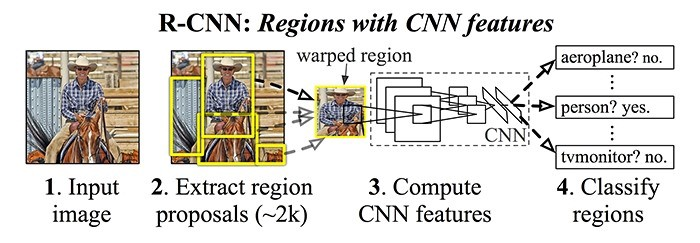
\includegraphics[width=0.6\columnwidth]{classification_based_algorithms}
		\caption{Detection using R-CNN (A classification based algorithm).}\label{fig:class-algos}
	\end{figure}
	\item \textbf{Regression-based algorithms} (aka \textit{Single Stage Detectors}): these types of algorithms are faster then the above algorithms, in that there is no selection of the ROI, so that the bounding boxes and the labels are predicted for the whole image at once; they are able to identify and classify objects within the image at once.
	\begin{itemize}
		\item beyond the higher speed, a key point is that the predictions are informed by the global context in the image, thus they generally lead to higher accuracies.
	\end{itemize}
	\begin{figure}[H]
		\centering
		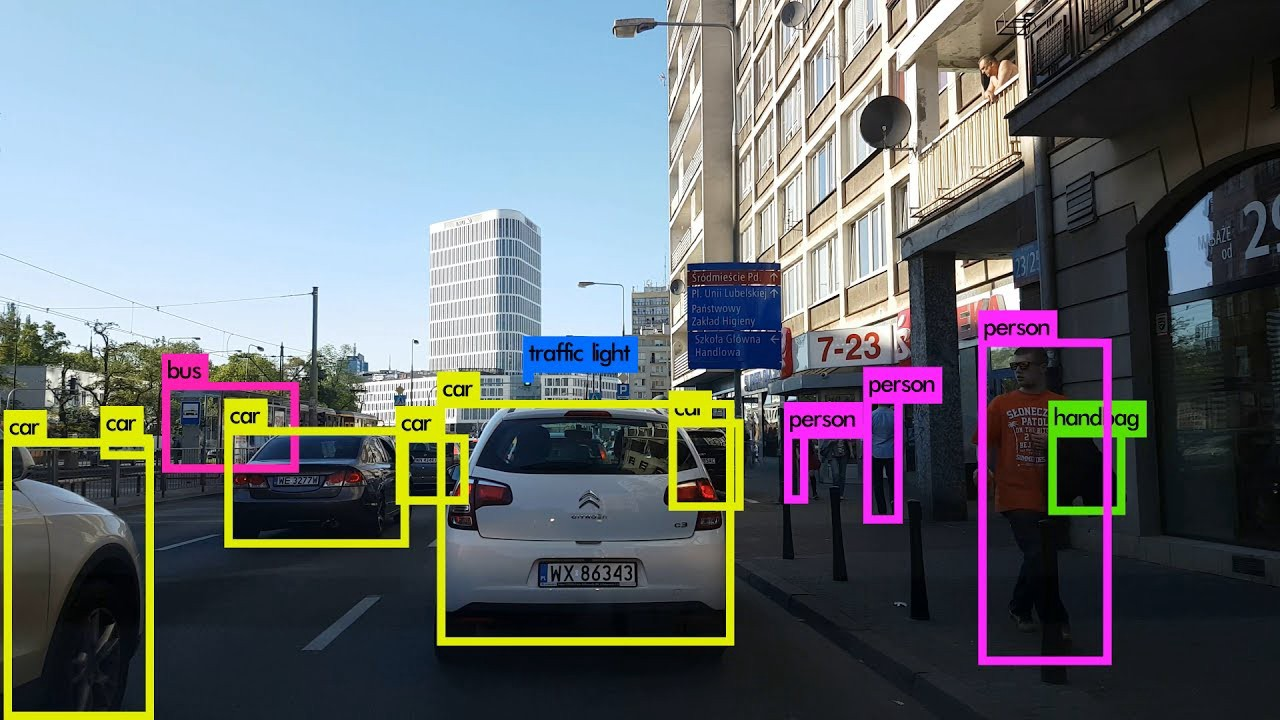
\includegraphics[width=0.6\columnwidth]{regression_based_algorithms}
		\caption{Detection using YOLO (A regression based algorithm).}\label{fig:regr-algos}
	\end{figure}
\end{itemize}
\noindent
YOLO, as its acronym reveals (You Only Look Once), falls into the regression-based algorithms: it applies a single neural network to the full image. In a nutshell, this network divides the image into regions and predicts bounding boxes and probabilities for each region. These bounding boxes are weighted by the predicted probabilities: in detail, each bounding box has a corresponding confidence score of how accurate it assumes that prediction should be and detects only one object per bounding box. The boundary boxes are generated by clustering the dimensions of the ground truth boxes from the original dataset to find the most common shapes and sizes.\\
\noindent
Since it makes predictions with a single network evaluation, it is extremely fast, more than 1000x faster than \textit{R-CNN} (which requires instead thousands of network evaluations for a single image) and 100x faster than \textit{Fast R-CNN}.

\subsection{YOLO history and milestones}\label{ss:yolo-history}
YOLO is originally introduced by Joseph Redmon in Darknet: Darknet is an open source library written in C and CUDA (thus supports CPU and GPU computation) by Joseph Redmon himself in order to ease the process of implementing YOLO and other object detection models.\
YOLO’s first version breaks the competition over R-CNN and DPM (Deformable Parts Model) thanks to:
\begin{itemize}
	\item real-time frames processing at 45 FPS;
	\item less false positives on the background;
	\item higher detection accuracy (although lower accuracy on localization).
\end{itemize}
\noindent
The algorithm has continued to evolve ever since its initial release in 2016. Both YOLO v2 and YOLO v3 were written by Joseph Redmon. After YOLO v3, there came new authors who anchored their own goals in every other YOLO release.\\
\noindent
In summary:
\begin{enumerate}
	\item \textbf{YOLO v2}: released in 2017, this version earned an honorable mention at CVPR 2017 because of significant improvements on anchor boxes, batch normalization and higher resolution.
	\item \textbf{YOLO v3}: the 2018 release had an additional objectness score to the bounding box prediction and connections to the backbone network layers. It also provided an improved performance on tiny objects because of the ability to run predictions at three different levels of granularity.
	\item \textbf{YOLO v4}: April’s release of 2020 became the first paper not authored by Joseph Redmon. Here Alexey Bochkovski introduced novel improvements, including mish activation, improved feature aggregation, etc.
	\item \textbf{YOLO v5}: Glenn Jocher continued to make further improvements in his June 2020 release, focusing on the architecture itself: however, this release is not published yet, it is still considered in progress.
\end{enumerate}
\noindent
We decided to re-implement in PyTorch the 3rd version since it is well-documented and widely tested by several computer vision communities: there are not many works and experiments with regard to the 4th version yet and there is not a scientific paper regarding the 5th version.

\subsection{YOLO architectures at a glance}\label{ss:arch-glance}
YOLO v2 used a custom deep architecture \textit{darknet-19}\footnote{\textit{Darknet-$n$} refers to a convolutional neural network which is $n$ layers deep.}, an originally 19-layer network supplemented with 11 more layers for object detection.\
With a 30-layer architecture, YOLO v2 often struggled with small object detections: this was attributed to loss of fine-grained features as the layers downsampled the input. To remedy this, YOLO v2 used an identity mapping, concatenating feature maps from a previous layer to capture low level features.\
However, YOLO v2’s architecture was still lacking some of the most important elements that are now staple in most of state-of-the art algorithms, such as residual blocks, skip connections and upsampling: YOLO v3 incorporates all of these.\
First, YOLO v3 uses \textit{Darknet-53} as its backbone\footnote{Backbone is not a universal technical term in deep learning and it has mainly two meaning: it can refer to the feature extraction part of the network or, more trivially, to the crucial part of the overall architecture.}, which, as the name reveals, has a 53 layer network trained on Imagenet: for the task of detection, 53 more layers are stacked onto it, leading to a 106 layer fully convolutional underlying architecture for YOLO v3. This is the reason behind the slowness of YOLO v3 compared to YOLO v2.\
The table below shows its higher efficiency with reference to competing backbones (ResNet-101 or ResNet-152).

\begin{figure}[H]
	\centering
	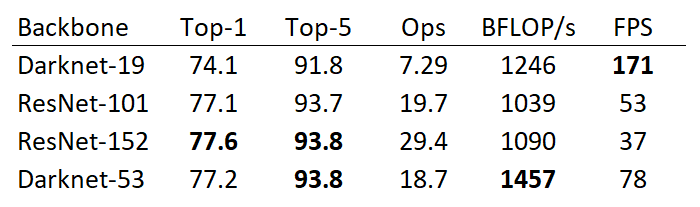
\includegraphics[width=0.6\columnwidth]{comparison}
	\caption{Comparison of backbones. Accuracy, billions of operations (Ops), billion floating-point operations per second (BFLOP/s), and frames per second (FPS) for various networks.} \label{fig:comparison}
\end{figure}
\noindent
Darknet-53 is 1.5 times faster than ResNet-101 and 2 times faster than ResNet-152, without entailing any trade-off in terms of accuracy and speed, since it is still as accurate as ResNet-152.\\
\noindent
YOLO v3 is fast and accurate in terms of mean average precision (mAP) and intersection over union (IoU) values as well. It runs significantly faster than other detection methods with comparable performance.

\begin{figure}[H]
	\centering
	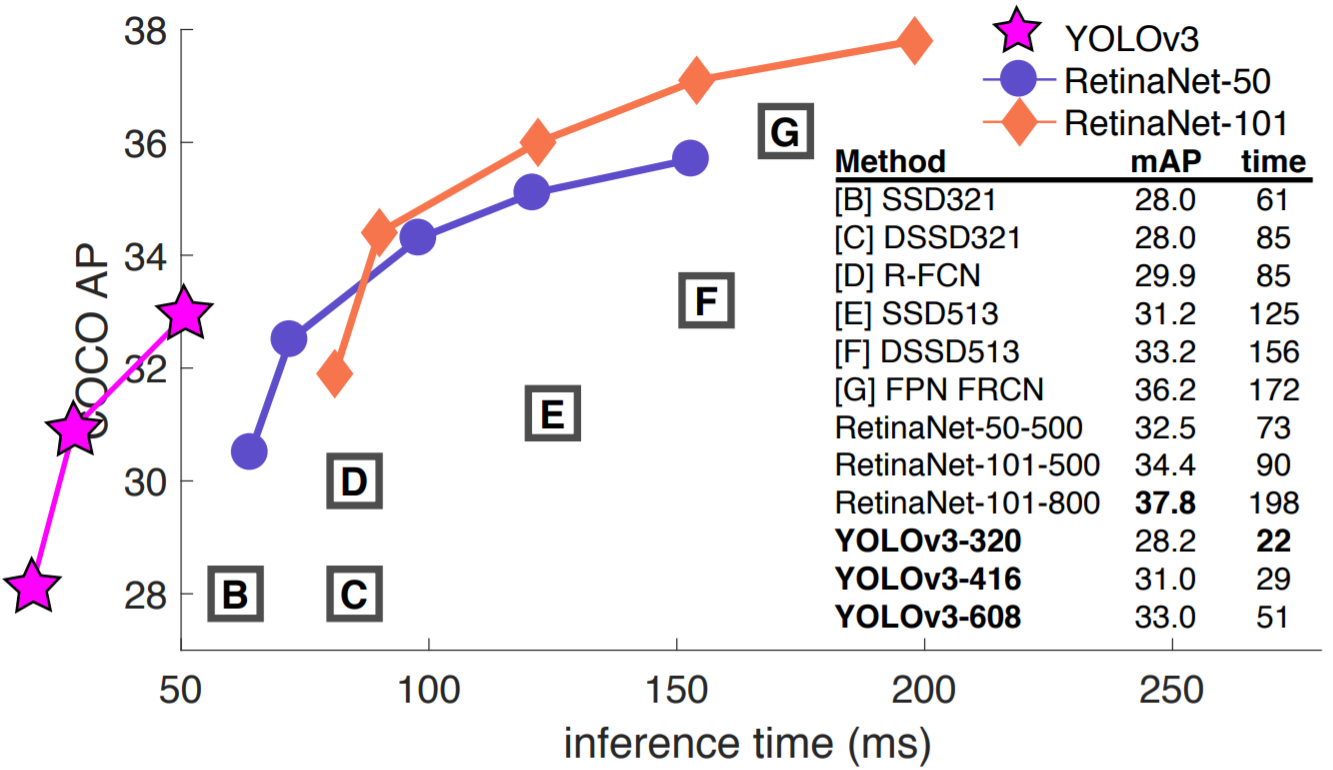
\includegraphics[width=0.6\columnwidth]{inference_times}
	\caption{Comparison between YOLO v3 and other algorithms in terms of inference time.} \label{fig:inference-time}
\end{figure}
\noindent
As the above graph highlights, YOLO v3 runs much faster than other detection methods with a comparable performance using an M40/Titan X GPU.

\section{Network blocks}\label{s:network-blocks}
In order to re-implement YOLO v3 in PyTorch, first of all, we analyzed \href{https://github.com/pjreddie/darknet/blob/master/cfg/yolov3.cfg}{Darknet's \texttt{yolov3.cfg} configuration file} to look out for patterns.\
The original network configuration has five different types of blocks, of which:
\begin{itemize}
    \item \textbf{convolutional} blocks which stand for plain convolutional layers to be added to the network (with some given hyperparameters), followed by a batch normalization layer and a Leaky ReLU activation function;
    \item \textbf{shortcut} blocks performing residual connections;
    \item \textbf{yolo} blocks doing nothing more than transforming the input: indeed, these are the blocks devoted to computing the loss value at the three output scales;
    \item \textbf{route} blocks which either return the output of some previous layer (this scenario happens after each \textbf{yolo} block) or perform a concatenation of outputs of two previous layers;
    \item \textbf{upsample} blocks that stand for plain upsample layers to be added to the network.
\end{itemize}
A deeper analysis of the network configuration allows to extract an easier representation of it and therefore an easier customization.\\
Our developed network configuration has the following blocks:
\begin{itemize}
    \item \textbf{convolutional}, which are equal to the convolutional blocks of the previous configuration;
    \item \textbf{residual}, which are a combination of two consecutive \textbf{convolutional} blocks followed by a residual connection (i.e., the previous \textbf{shortcut} block), repeated as many times as required by the block's hyperparameters;
    \item \textbf{scale prediction}, which are a combination of one \textbf{convolutional} \textit{block} and one \textbf{convolutional} block without the batch normalization and Leaky ReLU (i.e., a plain convolutional layer) in which the latter outputs a tensor with all the data for computing the loss and performing the object detection;
    \item \textbf{detection}, which are a combination of three \textbf{convolutional} blocks and a \textbf{scale prediction} block.
    This last block is excluded from the forward pass in order not to need, as for the previous network configuration, a \textbf{route} block returning the output of its predecessor.
\end{itemize}

\subsection{Convolutional}\label{ss:network-blocks-convolutional}
As we briefly described earlier, the \textbf{convolutional} block represents a concatenation of three layers:
\begin{itemize}
    \item a \textbf{two-dimensional (2D) convolutional} layer (two dimensions since we are dealing with images);
    \item a \textbf{batch normalization} layer;
    \item a \textbf{Leaky ReLU} as activation function.
\end{itemize}
We shall regard these layers as the function $$ConvBlock(x) \; \stackrel{def}{=} \; LeakyReLU(BatchNorm(Conv2d(x))).$$
\begin{figure}[h]
    \centering
    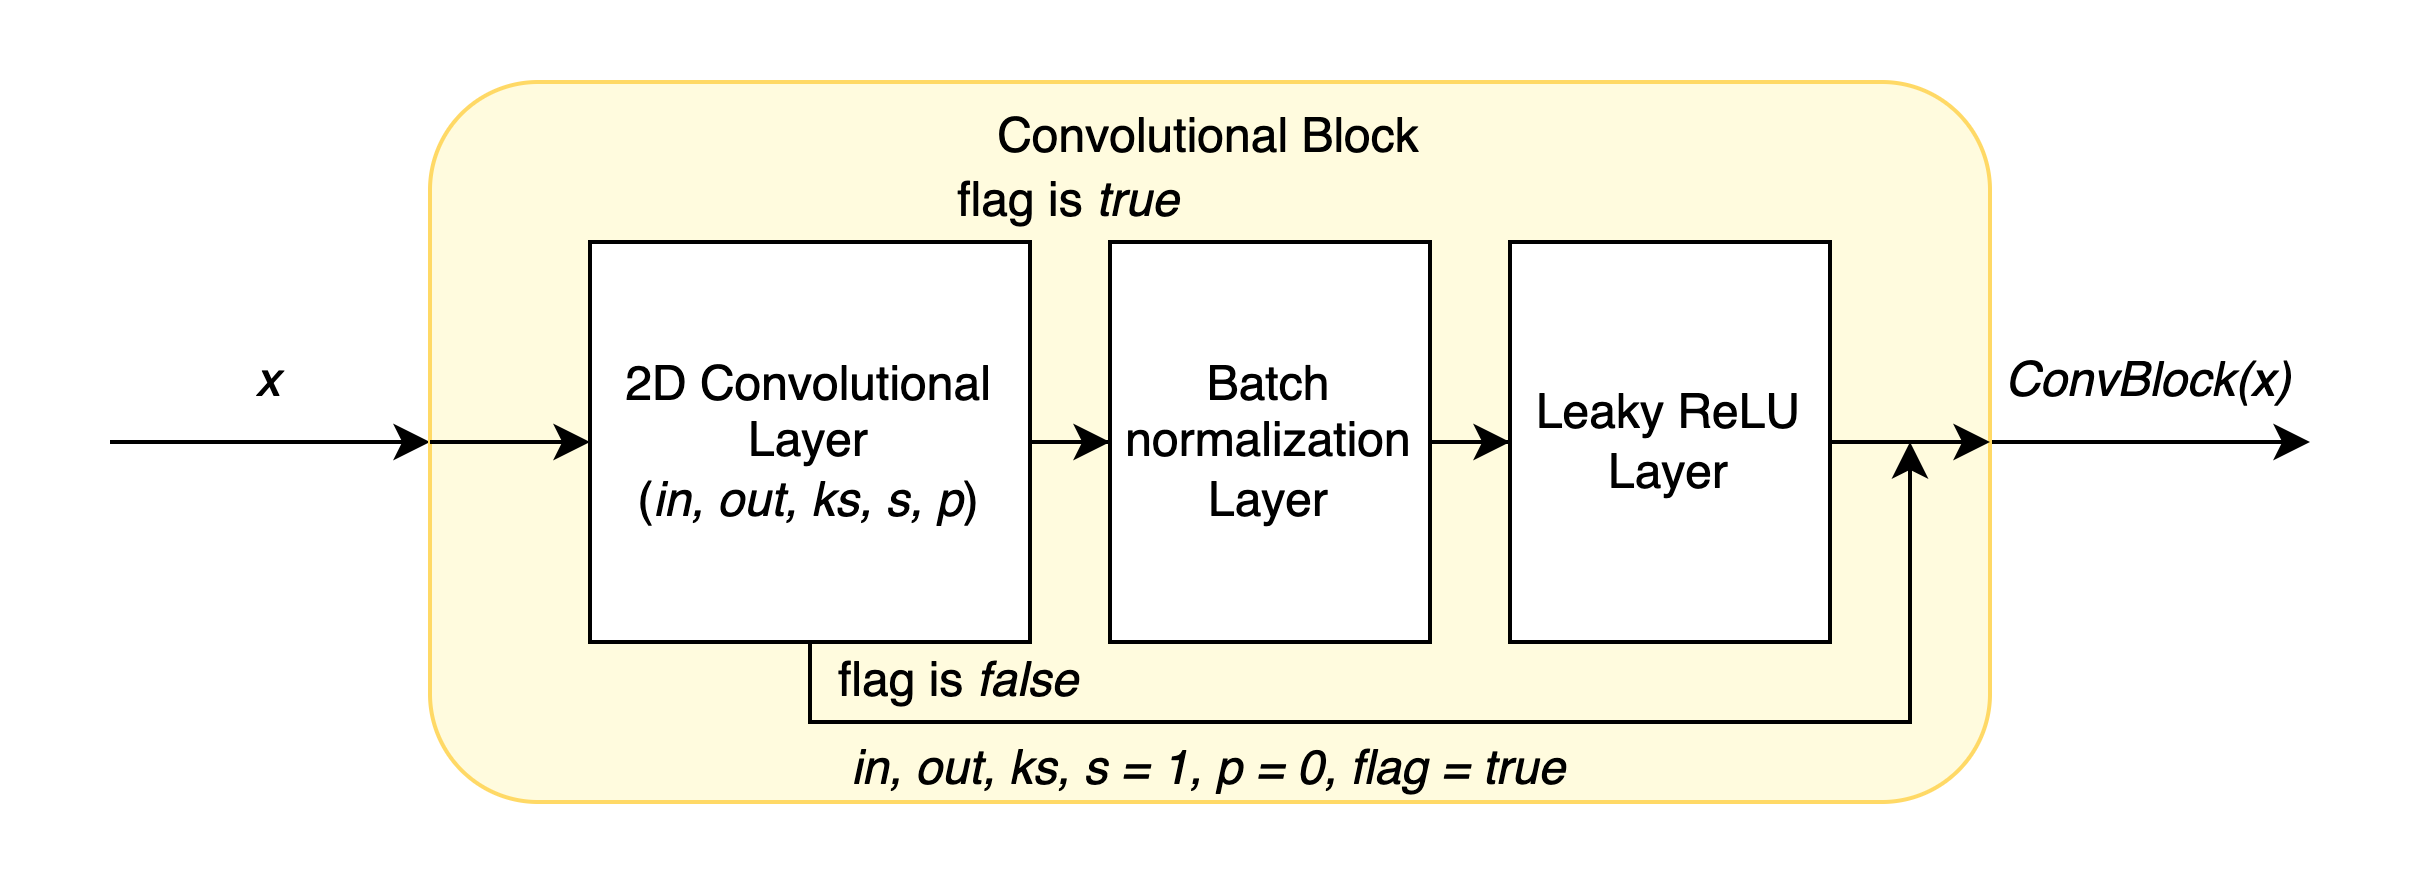
\includegraphics[width=0.65\textwidth]{assets/images/convolutional_block}
    \caption{Convolutional block: graphical representation}\label{img:convolutional_block}
\end{figure}\\
For this block we require the following hyperparameters:
\begin{itemize}
    \item the \textbf{number of input channels} $in$ which, in the case of the first block of the network, is the number of color channels of the input image;
    \item the \textbf{number of output channels} $out$ which generally corresponds to the number of convolutional kernels to be learned and to the number of values to be predicted when they are found last inside a \textbf{scale prediction} block;
    \item the \textbf{convolutional kernel size} $ks$ representing a kernel of receptive field $ks\times{}ks$, hence dimensions $ks\times{}ks\times{}in$;
    \item the \textbf{padding} $p$, with a default value of $0$, to apply both to the width and to the height;
    \item the \textbf{stride} $s$, with a default value of $1$;
    \item a boolean flag, \textit{flag}, with a default value of \texttt{true}, which controls whether to add a batch normalization layer and a Leaky ReLU activation function after the 2D convolutional layer (of course, when the flag is \texttt{false} then $ConvBlock(x) \; \stackrel{def}{=} \; Conv2d(x)$).\newline    
	In order to distinguish between the two, sometimes we will use the notations $ConvBlock_{batch}(x)$ and $ConvBlock_{nobatch}(x)$.
\end{itemize}
Given the input $x$, the forward pass returns $ConvBlock(x)$.

\subsection{Residual}\label{ss:network-blocks-residual}
A \textbf{residual} block, as we briefly described earlier, is nothing more than two \textbf{convolutional} blocks $ConvBlock_1$, $ConvBlock_2$ with a residual connection, repeated a fixed amount of times $n$.\\
One important detail about this block is that the shape of the output tensor from the two \textbf{convolutional} blocks is kept equal to that of the input, in order to sum residuals component-wise.
This is done by the first block having the output channels $out_1 = \frac{in_1}{2}$, a stride $s_1 = 1$, a padding $p_1 = 0$, and a kernel size $ks_1 = 1$;
the second block having $in_2 = out_1$, $s_2 =1$, $p_2 = 1$ and $ks_2 = 3$.\\
Let's regard this block as the function 
$$ResBlock_n(x) \; \stackrel{def}{=} \;
\begin{cases}
    ResBlock_{n-1}(x) \; + \; ConvBlock_{n,2}(ConvBlock_{n,1}(ResBlock_{n-1}(x))), & n > 1 \\
    x & n = 1
\end{cases}$$
with $n$ the number of repetitions, yielding a total amount of $2n$ \textbf{convolutional blocks} and $n$ residual connections.
\begin{figure}[h]
    \centering
    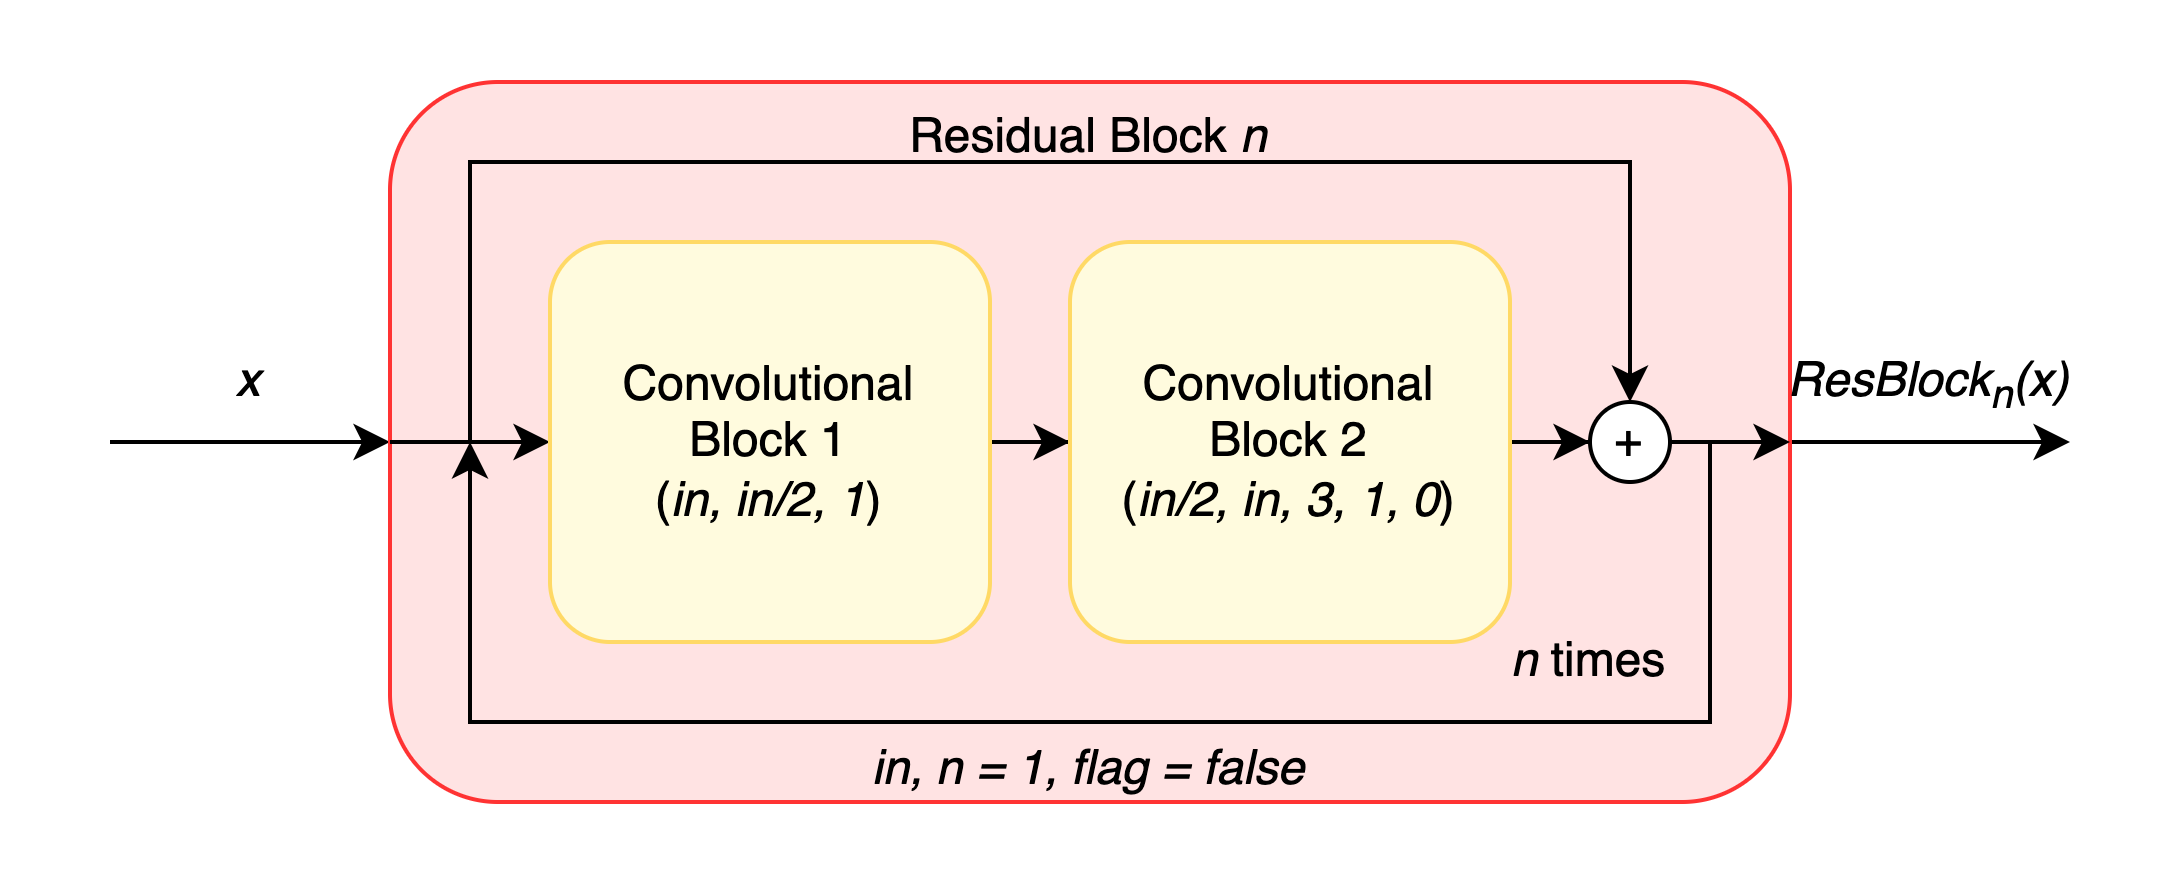
\includegraphics[width=0.65\textwidth]{assets/images/residual_block}
    \caption{Residual block: graphical representation}\label{img:residual_block}
\end{figure}\\
The hyperparameters for this block are:
\begin{itemize}
    \item the \textbf{number of input channels} $in$ ($= in_1$), which needs to match the number of output channels of the previous block;
    \item the \textbf{number of repetitions} $n$ (default value of $1$), which is the number of times the couple of \textbf{convolutional} blocks needs to be added to the block list of the network;
    \item a boolean flag, \textit{flag}, with a default value of \texttt{false}, for saving the output of the block to perform a route connection (which is what was done by the \textbf{route} block in the previous configuration).
\end{itemize}
Given the input $x$, the forward pass returns $ResBlock_n(x)$ and if the flag is set to \texttt{true}, the returned value is stored by the network for later use.

\subsection{Scale prediction}\label{ss:network-blocks-scale-prediction}
This is a special block because its output does not contribute to the network itself but only to the loss function value, which is explained in \hyperref[s:loss-function]{Section 3.4}.
In the whole network there are just three of these blocks and each one contributes to one third of the loss, namely $\ell_i$, with $i \in{} {\{1,2,3\}}$.\\
It is composed by a first \textbf{convolutional} block $ConvBlock_{batch}$ with $out_{batch} = 2in_{batch}$, $s_{batch} = 1$, $p_{batch} = 1$, $ks_{batch} = 3$ and a second \textbf{convolutional} block $ConvBlock_{nobatch}$ with $out_{batch} = (5 \; + \; \#classes) \; \cdot{} \; \#anchors_i$, $s_{nobatch} = 1$, $p_{nobatch} = 0$, $ks_{nobatch} = 1$, without the batch normalization and Leaky ReLU.\\
For the ImageNet dataset, for instance, $\#classes = 1000$ and $\#anchors_i = 3$ $\forall{} i \in{} {\{1,2,3\}}$.\\
This block can be represented by the function $$ScalePredBlock(x) \; \stackrel{def}{=} \; ConvBlock_{nobatch}(ConvBlock_{batch}(x)).$$
\begin{figure}[h]
    \centering
    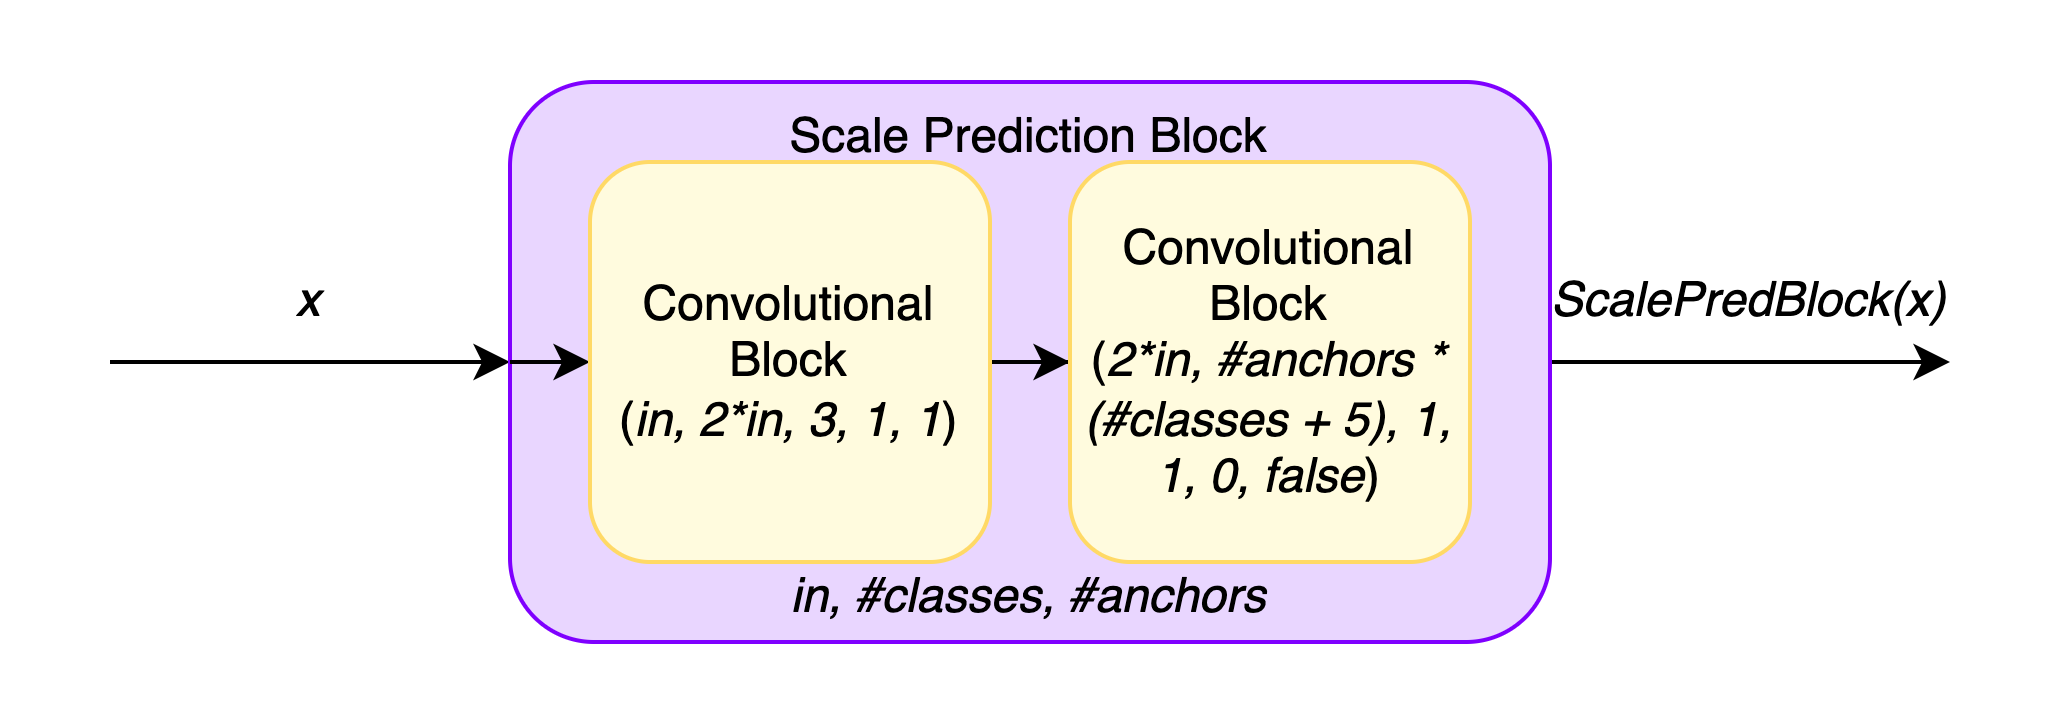
\includegraphics[width=0.65\textwidth]{assets/images/scaleprediction_block}
    \caption{Scale Prediction block: graphical representation}\label{img:scaleprediction_block}
\end{figure}\\
The hyperparameters are:
\begin{itemize}
    \item the \textbf{number of input channels} $in$ ($= in_{batch}$), which needs to match the number of output channels of the previous block;
    \item the \textbf{number of classes} $\#classes$ of the dataset which need to be predicted;
    \item the \textbf{number of anchors} $\#anchors$ of the dataset for the scale level $i$ which the block predicts the loss for.
\end{itemize}
Please note that even if our implementation allows to set $\#anchors$ for each scale, we decided to stick with the original idea of having three anchors per \textbf{scale prediction} block as in the original implementation ($\#anchors_i = 3$ $\forall{} i \in{} {\{1,2,3\}}$, as we said earlier).\\
Given the input $x$, the forward pass outputs $y^{\prime\prime}$, which is:
$$y^{\prime\prime} = (y^\prime_1 \; y^\prime_2 \; y^\prime_4 \; y^\prime_5 \; y^\prime_3) \; \text{with $y^\prime_i$ the $i$-th column of $y^\prime$},$$
$$y^\prime = reshape_{(batch\_size,\ \#anchors,\ 5 \; + \; \#classes,\ grid\_size,\ grid\_size)}(ScalePredBlock(x)),$$
considering $x$ having an original shape of $batch\_size \times{} \dots{} \times{} grid\_size \times{} grid\_size$.

\subsection{Upsample}\label{ss:network-blocks-upsample}
This block is merely a wrapper around an upsample layer, with \textbf{bilinear} as the upsampling algorithm.
This block can be represented with the function
$$UpsampleBlock(x) \; \stackrel{def}{=} \; Upsample(x).$$
\begin{figure}[h]
    \centering
    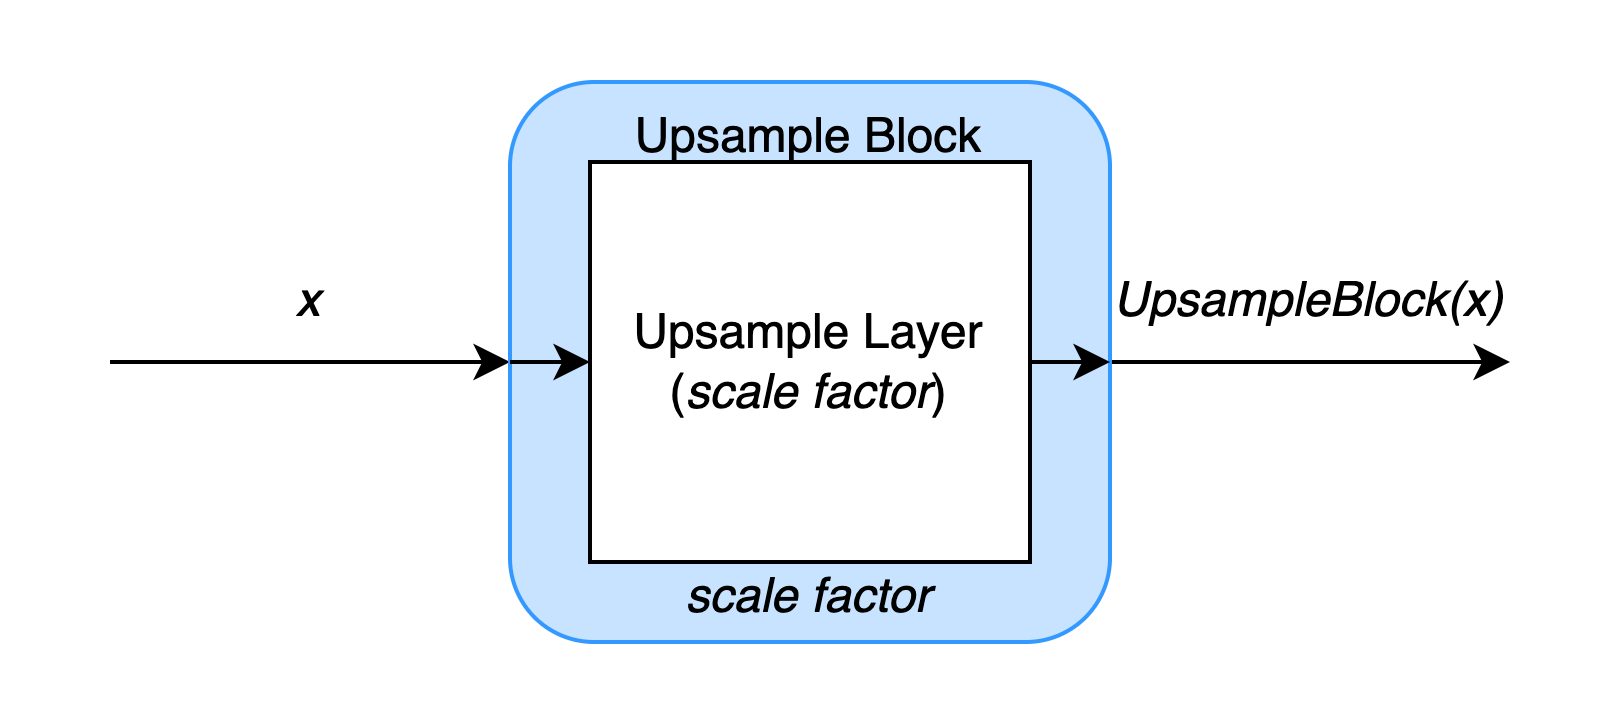
\includegraphics[width=0.65\textwidth]{assets/images/upsample_block}
    \caption{Upsample block: graphical representation}\label{img:upsample_block}
\end{figure}\\
There is just one hyperparameter, which is the \textbf{scale factor}, namely the factor used for increasing the last axis dimensions of the input tensor.\\
Given the input $x$, the forward pass outputs $UpsampleBlock(x)$ and the network updates the current output tensor with the concatenation of $UpsampleBlock(x)$ and the output of the last $ResBlock_n(x)$ with the flag set to \texttt{true}.

\subsection{Detection}\label{ss:network-blocks-detection}
This last block we are describing performs the final steps before having the partial loss $\ell_i$, with $i \in{} {\{1,2,3\}}$, as the result of the \textbf{scale prediction} block.\\
It is made of three \textbf{convolutional blocks}, the first two acting exactly like those in the \textbf{residual} block but without the summation of $x$; the third performing $1\times{}1$ convolutions, preparing the input for the \textbf{scale prediction} block.\\
A function representing this block can be
$$DetectionBlock(x) \; \stackrel{def}{=} \; ConvBlock_3(ConvBlock_2(ConvBlock_1(x))).$$
\begin{figure}[h]
    \centering
    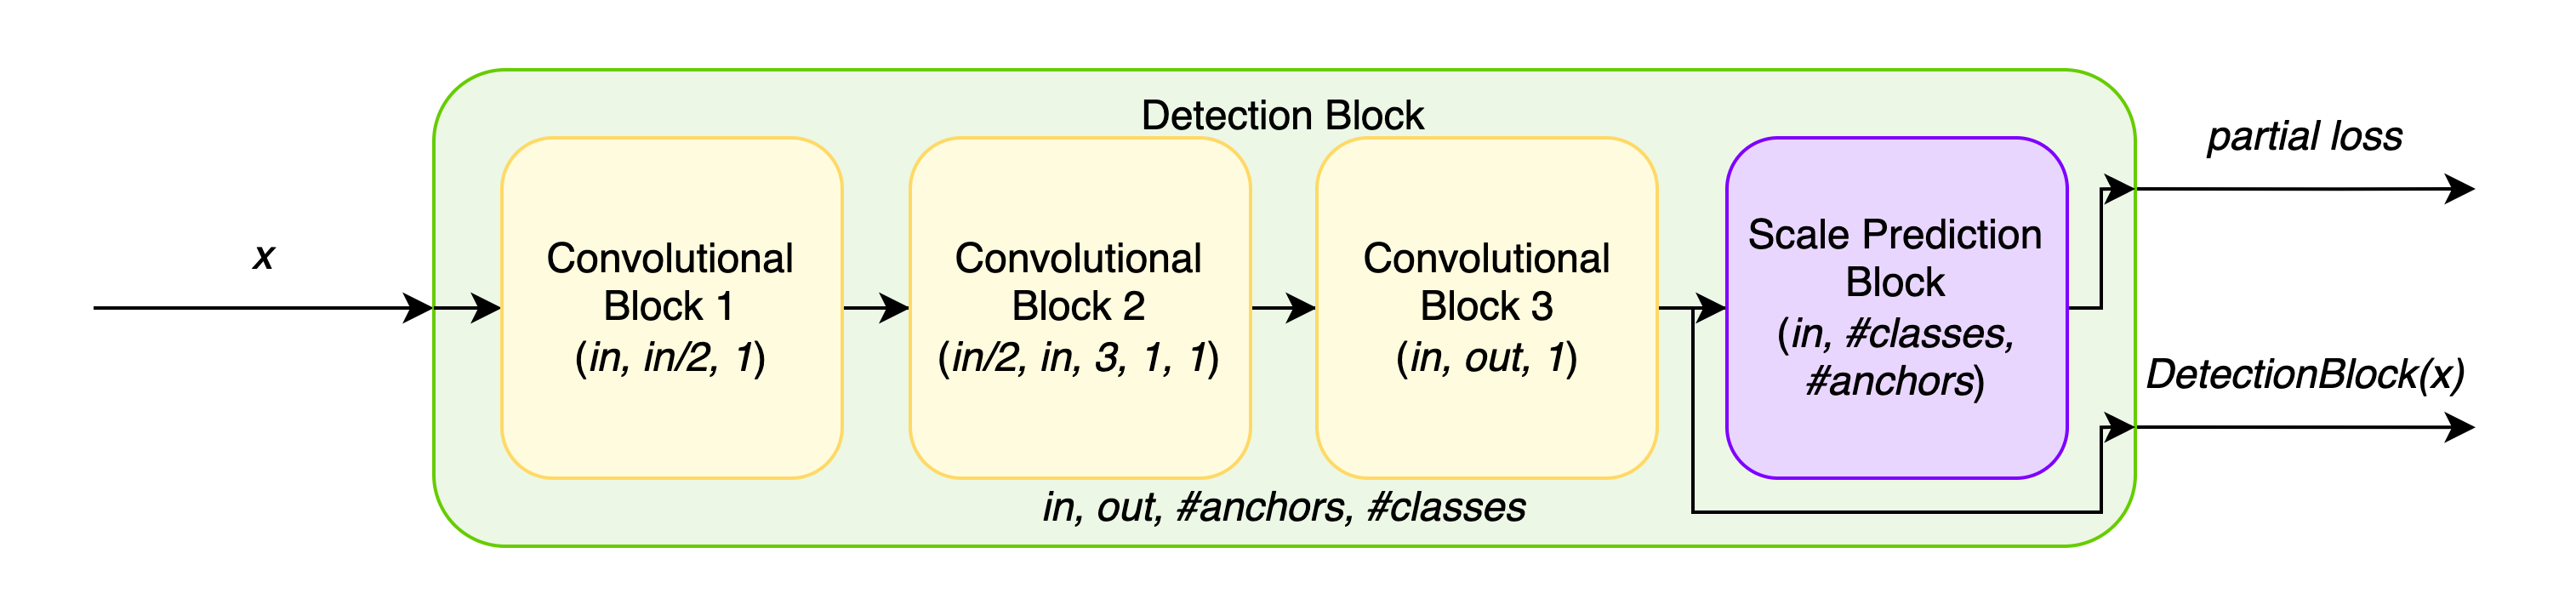
\includegraphics[width=0.85\textwidth]{assets/images/detection_block}
    \caption{Detection block: graphical representation}\label{img:detection_block}
\end{figure}\\
The hyperparameters are the following:
\begin{itemize}
    \item the \textbf{number of input channels} $in$, which needs to match the number of output channels of the previous block;
    \item the \textbf{number of output channels} $out$, that is the number of convolutional kernels to be learned and the input channels for the \textbf{scale prediction} block;
    \item the \textbf{number of classes} $\#classes$ of the dataset which need to be predicted (forwarded to the \textbf{scale prediction} block);
    \item the \textbf{number of anchors} $\#anchors$ of the dataset for the scale the block predicts the loss for (forwarded to the \textbf{scale prediction} block).
\end{itemize}
Given input $x$, the forward pass outputs $y = DetectionBlock(x)$ and the network computes the partial loss $\ell_i = ScalePredBlock(y)$.

\newpage
\section{Network layout}\label{s:network-layout}
With the blocks defined in the previous section, we present the base architecture of the YOLO v3 network.
\begin{figure}[!h]
    \centering
    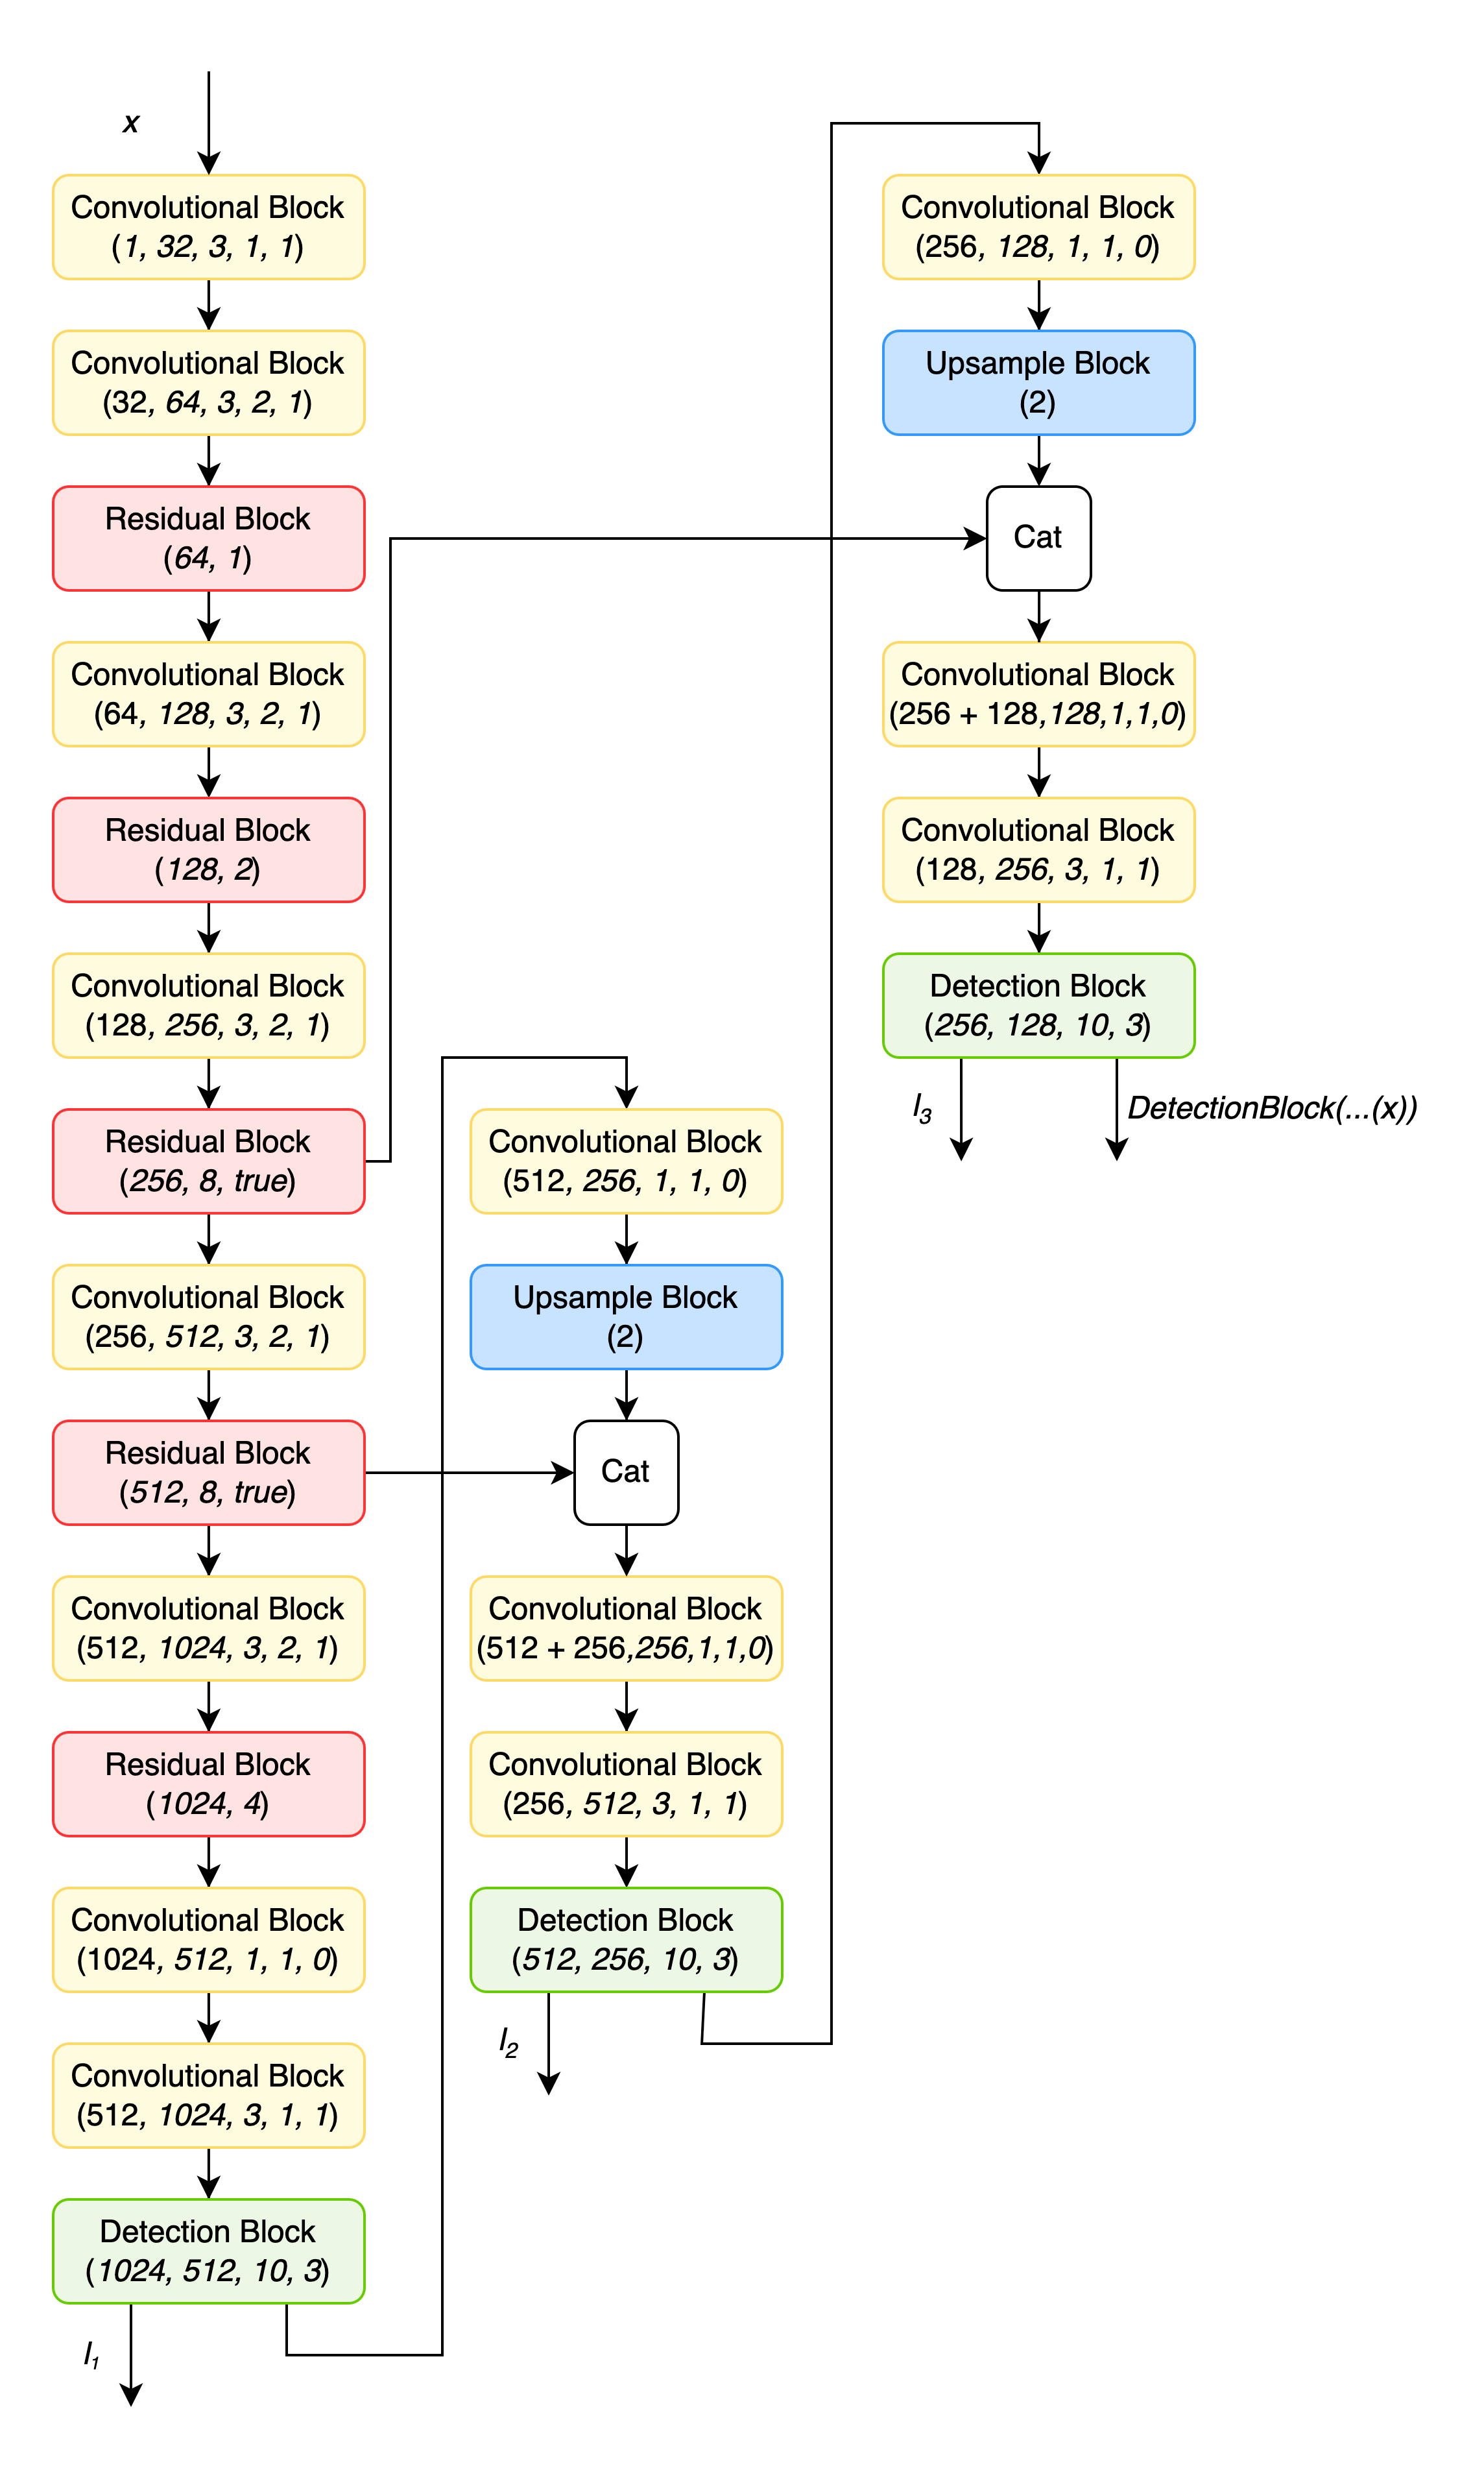
\includegraphics[width=0.47\textwidth]{assets/images/network_base}
    \caption{YOLO v3 base network architecture: graphical representation}\label{img:yolo_v3_base_network_architecture}
\end{figure}\\
This architecture respects the specification of the original YOLO v3 architecture.
As we will describe in the \hyperref[c:tests-and-results]{following section}, some adjustments were made to improve the convergence speed.
In the diagram we clearly notice what we described in the previous sections:
\begin{itemize}
    \item first of all, we notice that at the end of each of three ``column of blocks" there is a \textbf{detection block} which returns the output tensor $DetectionBlock(\dots(x))$ and $\ell_i$;
    \item there are two \textbf{residual} blocks which have the boolean flag set to \texttt{true} and indeed their value is stored inside the network, as it is shown, to be concatenated with the output of the two \textbf{upsample} blocks;
    \item the downsampling, as we briefly described in \hyperref[ss:yolo-history]{Section 3.1.1} and \hyperref[ss:arch-glance]{Section 3.1.2}, which takes an input image of size $w \times{} h$ and reduces it by factors $2^5$, $2^4$, $2^3$ (these are obtained by multiplying the stride of all the \textbf{convolutional} blocks until each \textbf{detection} block) to obtain three \textbf{feature maps} at three different recognition scales (which discover progressively smaller objects).
    With our dataset, it means that the input images of size $128\times{}128$ gets transformed to three feature maps of sizes $4\times{}4$, $8\times{}8$, $16\times{}16$.
\end{itemize}

\section{Loss function}\label{s:loss-function}
The loss function of the network is quite complex since it needs to consider many aspects:
\begin{itemize}
    \item the bounding boxes, which are described by their width $w$, height $h$, center coordinates $(x, y)$;
    \item the objectness score, which describes how much a given bounding box is likely to be recognizing an object;
    \item the no-objectness score, which describes how much a given bounding box is likely \textit{not} to be recognizing an object;
    \item the class probabilities, which describe how likely it is that the bounding box is recognizing an object of each class.
\end{itemize}
Moreover, the final loss value $\ell$ is obtained by summing the three partial losses, hence $\ell{} = \sum_{i=1}^{3}{\ell_i}$.\newline
The output of $ScalePredBlock$, at each scale $i$, is a tensor $\hat{out}$ of shape $(batch\_size,$ $\#anchors_i,$ $grid\_size_i,$ $grid\_size_i,$ $5 + \#classes)$, 
while the corresponding target $out$ has shape $(batch\_size,$ $\#anchors_i,$ $grid\_size_i,$ $grid\_size_i,$ $5+1)$.\\
Please note that, for the sake of simplicity, we will not consider the $batch\_size$ in the loss formula (we shall regard it as $batch\_size = 1$). It would only add further summation and additional subscript index.
Finally, the loss function at this scale is the following:
\begin{align*}
    \ell_i &= \lambda_{noobj} \cdot{} 
    \displaystyle\sum_{k=1}^{A}{
        \displaystyle\sum_{i=1}^{S}{
            \displaystyle\sum_{j=1}^{S}{
                \mathbbm{1}_{k,i,j}^{noobj} \; \frac{LogLoss(\sigma(\hat{c}_{k,i,j}), c_{k,i,j}))}{\#noobjects}
            }
        }
    } & \text{(no object loss)}\\
    &+ \lambda_{obj} \cdot{} 
    \displaystyle\sum_{k=1}^{A}{
        \displaystyle\sum_{i=1}^{S}{
            \displaystyle\sum_{j=1}^{S}{
                \mathbbm{1}_{k,i,j}^{obj} \; \frac{SquaredError(\sigma(\hat{c}_{k,i,j}), IoU(\hat{obj\_bbox}_{k,i,j}, obj\_bbox_{k,i,j}))}{\#objects}
            }
        }
    } & \text{(object loss)}\\
    &+ \lambda_{box} \cdot{} 
    \displaystyle\sum_{k=1}^{A}{
        \displaystyle\sum_{i=1}^{S}{
            \displaystyle\sum_{j=1}^{S}{
                \mathbbm{1}_{k,i,j}^{obj} \; \frac{SquaredError(\hat{bbox}_{k,i,j}, bbox_{k,i,j})}{\#objects}
            }
        }
    } & \text{(box loss)}\\
    &+ \lambda_{class} \cdot{} 
    \displaystyle\sum_{k=1}^{A}{
        \displaystyle\sum_{i=1}^{S}{
            \displaystyle\sum_{j=1}^{S}{
                \mathbbm{1}_{k,i,j}^{obj} \; \frac{LogSoftmax_C(\hat{p}_{k,i,j}, p_{k,i,j})}{\#objects}
            }
        }
    } & \text{(class loss)}\\
\end{align*}
with:
\begin{itemize}
    \item $A=\#anchors_i$
    \item $S=grid\_size_i$
    \item $C=\#classes$
    \item $anchor_i = [anchor\_w \; \; anchor\_h]$
    \item $\forall{} k \in [1,A], \; i, j \in [1,S] \; \mathbbm{1}_{k,i,j} = \begin{cases}
        1 & \text{bbox contains an object and has the highest IoU at scale $k$}\\
        -1 & \text{bbox contains an object but does not have the highest IoU at scale $k$}\\
        0 & \text{otherwise}\\
    \end{cases}$
    \item $\#objects = \displaystyle\sum_{k=1}^{A}{\displaystyle\sum_{i=1}^{S}{\displaystyle\sum_{j=1}^{S}{(\mathbbm{1}_{k,i,j}^{obj} = 1)}}}$\footnote{\label{ft:note}This is a little abuse of notation: we mean ``return 1 when $\mathbbm{1}_{k,i,j}^{obj}$ equals 1 (or 0), 0 otherwise".}
    \item $\#noobjects = \displaystyle\sum_{k=1}^{A}{\displaystyle\sum_{i=1}^{S}{\displaystyle\sum_{j=1}^{S}{(\mathbbm{1}_{k,i,j}^{obj}}} = 0)}$\footnoteref{ft:note}
    \item $\forall{} k \in [1,A], \; i, j \in [1,S] \; \; \hat{out}_{k,i,j} = [\hat{c} \; \; \hat{x} \; \; \hat{y} \; \; \hat{w} \; \; \hat{h} \; \; \hat{p}]$, $\hat{p} = (p_1 \; \dots \; p_C)$
    \item $\forall{} k \in [1,A], \; i, j \in [1,S] \; \; out_{k,i,j} = [c \; \; x \; \; y \; \; w \; \; h \; \; p]$
    \item $LogLoss(x, y) = y \cdot{} log\;x + (1-y) \cdot{} log(1-x)$
    \item $SquaredError(x, y) = (x - y)^2$
    \item $LogSoftmax_C(x, y) = log \; \frac{exp(x_y)}{\sum_{c = 1}^{C}{exp(x_{classes_c})}}$
    \item $\hat{obj\_bbox}_{k,i,j} = [\sigma(\hat{x}_{k,i,j}) \; \; \sigma(\hat{y}_{k,i,j}) \; \; exp(\hat{w}_{k,i,j})\cdot{}anchor\_w_k \; \; exp(\hat{h}_{k,i,j})\cdot{}anchor\_h_k]$
    \item $obj\_bbox_{k,i,j} = [x_{k,i,j} \; \; \; y_{k,i,j} \; \; \; w_{k,i,j} \; \; \; h_{k,i,j}]$
    \item $\hat{bbox}_{k,i,j} = [\sigma(\hat{x}_{k,i,j}) \; \; \sigma(\hat{y}_{k,i,j}) \; \; \hat{w}_{k,i,j} \; \; \hat{h}_{k,i,j}]$
    \item $bbox_{k,i,j} = [x_{k,i,j} \; \; \; y_{k,i,j} \; \; \; log \; \frac{w_{k,i,j}}{anchor\_w_k} \; \; \; log \; \frac{h_{k,i,j}}{anchor\_h_k}]$.
\end{itemize}

\section{Network training}\label{s:network-training}

\subsection{Dataset}\label{ss:dataset}
Regarding datasets, we create the \texttt{DataLoader} objects for training, evaluation and testing.
\noindent
Moreover, we make use of the \textit{Automatic mixed precision package} offered by ``PyTorch": it allows to perform some operations by using the \texttt{torch.float32} (standard single precision floating point number) datatype and other operations by using \texttt{torch.float16} (half precision floating point number).\newline
Some operations, like linear layers and convolutions, are much faster in \texttt{float16}, while other ones, like reductions, often require the dynamic range of \texttt{float32}: mixed precision tries to match each operation to its appropriate datatype.

\subsection{Early stopping}\label{ss:early}
Our training process implements an \textbf{early stopping} mechanism: in the configuration file we set the tolerance regarding the number of epochs after which the specified metric does not improve.
Our specified metric is the mean loss value averaged over the batches needed to complete an epoch, namely the mean loss value during that epoch.\\
\noindent
We actually begin checking the evolution of the mean loss after the 5th epoch in order not to stop too early those training starting from a bad point in the loss function space.

\subsection{Performance measures}\label{ss:measures}
Regarding performance measures, we track the evolution of the \textit{class prediction accuracy}, the \textit{object accuracy}, the \textit{no object accuracy}, the \textit{mean loss} and the \textit{Mean Average Precision (mAP)}, over all the epochs: in detail, we plot on the same graph the evolution of every aforementioned metric during the training and the validation, so that they are able to highlight potential underfitting or overfitting.

\begin{figure}[h]
    \centering
    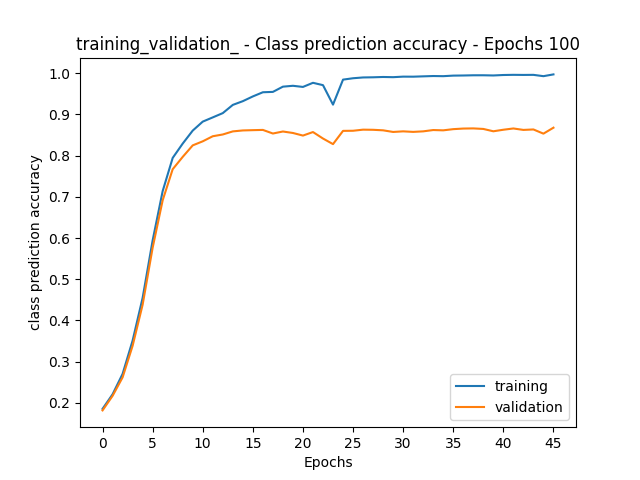
\includegraphics[width=0.85\textwidth]{assets/images/training_validation_Class_prediction_accuracy.png}
    \caption{Class prediction accuracy during training and validation steps.}\label{img:performances}
\end{figure}

\end{document}
